\documentclass[10pt]{article}

\usepackage[utf8]{inputenc}
\usepackage[T1]{fontenc}
\usepackage[english]{babel} % If needed, change language here
\usepackage{amssymb}
\usepackage{color}
\usepackage{graphicx}
\usepackage{caption}
\usepackage[obeyFinal]{easy-todo}
\usepackage{subcaption}

% Optional: decrease margins to fit more on one page
\usepackage{geometry}
\geometry{
	a4paper,
	total={190mm,257mm},
%	left=15mm,
%	top=15mm,
%	right=15mm,
%	bottom=15mm
}

% Place todo's using \todo
%\newcommand{\todo}{{\color{red}{\textbf{TODO }}}}



\begin{document}
\font\myfont=cmr12 at 15pt

\title{\vspace{-2.5cm}{\myfont Assignment 3: BDAP [B-KUL-H00Y4A]}}
\author{Andreas Hinderyckx}
\date{} % Choose custom date


\maketitle
%\listoftodos

\vspace{-1cm}
\paragraph{Question 1}
The approximate product quantization (PQ) method is faster than the naive nearest neighbors (NN) because it limits the amount of distance computations, which dominate execution time. Concretely: for naive NN $N$ distances are computed in the case of $N$ training examples. When using PQNN, the $N$ training instances are mapped onto \texttt{nclusters} $\ll N$ centroids. Only the distances between the query example and the \texttt{nclusters} must be calculated, hence the computation time drops significantly.

\vspace{-.3cm}
\paragraph{Question 2} The effect of \texttt{npartitions} and \texttt{nclusters} is shown in figure \ref{fig:hyperparams}.

\vspace{-.4cm}
\begin{figure}[h]
	\begin{subfigure}{.5\textwidth}
		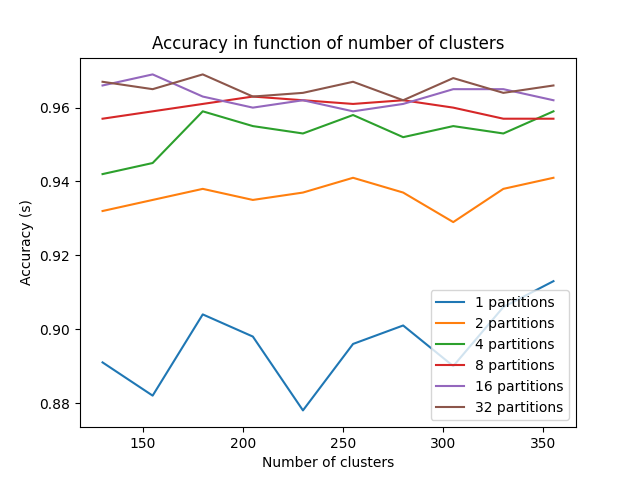
\includegraphics[width=\linewidth]{./img/Accuracy--covtype-hyp1-64--130-355.png}
		\caption{Accuracy}
		\label{fig:acc}
	\end{subfigure}%
	\hfill
	\begin{subfigure}{.5\textwidth}
		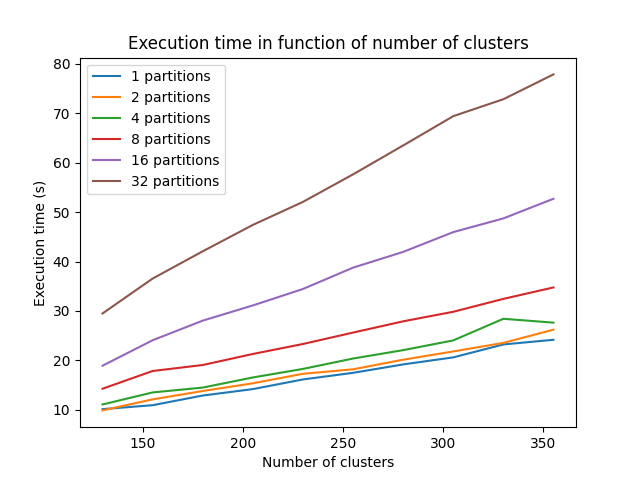
\includegraphics[width=\linewidth]{./img/Execution time--covtype-hyp1-64--130-355.png}
		\caption{Execution time}
		\label{fig:exec}
	\end{subfigure}
	\caption{Effect of number of clusters and number of partitions on accuracy (\ref{fig:acc}) and execution time (\ref{fig:exec}) of \texttt{ProdQuanNN} executed on the \texttt{covtype} dataset}
	\label{fig:hyperparams}
\end{figure}

\vspace{-.8cm}
\paragraph{Question 3} From figure \ref{fig:exec} it can be seen that the execution time grows linearly with the number of partitions and the number of clusters.

\end{document}
